\documentclass[margin,letterpaper,11pt]{scrartcl}
\usepackage[utf8]{inputenc}
\usepackage{graphicx}
\usepackage{epstopdf}
\usepackage{tikz}
\setlength{\textwidth}{6.5in}
\setlength{\textheight}{9in}
\setlength{\oddsidemargin}{0in}
\setlength{\evensidemargin}{\oddsidemargin}
\setlength{\topmargin}{0in}
\setlength{\headsep}{0in}
\setlength{\headheight}{0in}
\setlength{\parindent}{0in}
\parskip 7.2pt

% figure width
\newlength \figwidth
\setlength \figwidth {0.8\textwidth}
% figure half width
\newlength \fighwidth
\setlength \fighwidth {0.4\textwidth}

\begin{document}

% paper size
\special{papersize=8.5in,11in}
\setlength{\pdfpageheight}{\paperheight}
\setlength{\pdfpagewidth}{\paperwidth}

\title{FallDown Screen Specification}
\subtitle{Project 09, CSCI 410}
\date{}
\author{Brandon Vargo}
\maketitle

\section{Overview}

FallDown is a simple game where the player, represented by a ball, falls down
an endless hole full of obstacles. If the player does not fall fast enough,
such as the case where the player encounters an obstacle and cannot move out of
the way in time, then the player dies. It is impossible to win.

\section{Use Case Scenarios}

Yong is stuck on the moon in a broken spaceship. Since it will be some time
before Congress can authorize money to retrieve Yong, he needs something to
do. The \textit{Elements of Computing Systems} course is born. The hack
computer platform is designed so that Yong can build the system using only
the parts he can scavenge from the circuit boards of the space capsule.

Inspired by the depth of the moon craters and the size of the rocks
surrounding the craters, Yong creates the FallDown game for his hack computer
platform. Not only must the game run on the homemade (well, moon-made)
computer, but it must also fill Yong with glee for months as the politicians
back on Earth squabble over funding for the rescue mission. As a result, the
game must be both simple and fun to play. In addition, it is impossible to win
the game; this way, Yong cannot beat the game and subsequently be bored
sitting on the moon without a game to play.

FallDown is better for Yong than other games, such as Galaxian, which
may incite violence in the hitherto-unseen population of moon
aliens.  Interstellar war would be exciting for Yong, as he would be on the
front lines, and the entire Department of Defense budget would be allocated
to the war effort, but interstellar war is also known to the state of
California to cause cancer. FallDown is a safer game to play, from a cancer
perspective, leading to its rating of E for Everyone (except moon rocks, for
which it is deadly). Galaxian is only rated E for Cockroaches due to the
cancer risks.

\section{Non-Goals}

\begin{itemize}
   \item Winning is not a goal. Unlike other games, this game does not make
      the user feel good about themselves thanks to easy levels that are
      trivial to win.  Also, if Yong were to win the game, then he would be
      bored sitting on the moon.
   \item As stated in the use case section, inciting interstellar war is also
      not a goal of this game.
\end{itemize}

\section{Program Flow}

\usetikzlibrary{shapes,arrows}

% Define block styles
\tikzstyle{block} = [rectangle, draw, fill=blue!20,
    text width=5em, text centered, rounded corners, minimum height=4em]
\tikzstyle{line} = [draw, -latex']

\begin{tikzpicture}[node distance = 3cm, auto]
    \node [block] (title) {title screen};
    \node [block, right of=title] (game) {game screen};
    \node [block, right of=game] (loser) {loser screen};
    \path [line] (title) -- (game);
    \path [line] (game) -- (loser);
\end{tikzpicture}

\section{Individual Screen Specifications}

\subsection{Title Screen}

The title screen is the first screen that the user sees. This screen displays
the name of the game, instructions for playing the game, and instructions for
starting the game. The user is able to press the enter key or the spacebar in
order to start the game.

\subsection{Game Screen}

The game screen is the main action screen that provides excitement to all
players.  There are two main actors on this screen: the ball and the
obstacles. The player is the ball, which is falling through the obstacles. The
``camera'' is in a reference frame that ``falls'' at a constant rate. As a
result, the obstacles appear to move toward the top of the screen. The ball
falls faster than the camera.

The player is able to move the ball left and right using the arrow keys.
Gravity affects the ball; after all, if there is no gravity, there is
no falling. The ball cannot move below the bottom of the screen, and
the ball cannot move through obstacles. As a result of not being
able to move through obstacles, the ball will be pushed upwards
as the platforms move toward the top of the screen. If the ball
moves off of the top of the screen, then the ball is squashed, and the player
dies.

\begin{figure}[!h]
   \begin{center}
      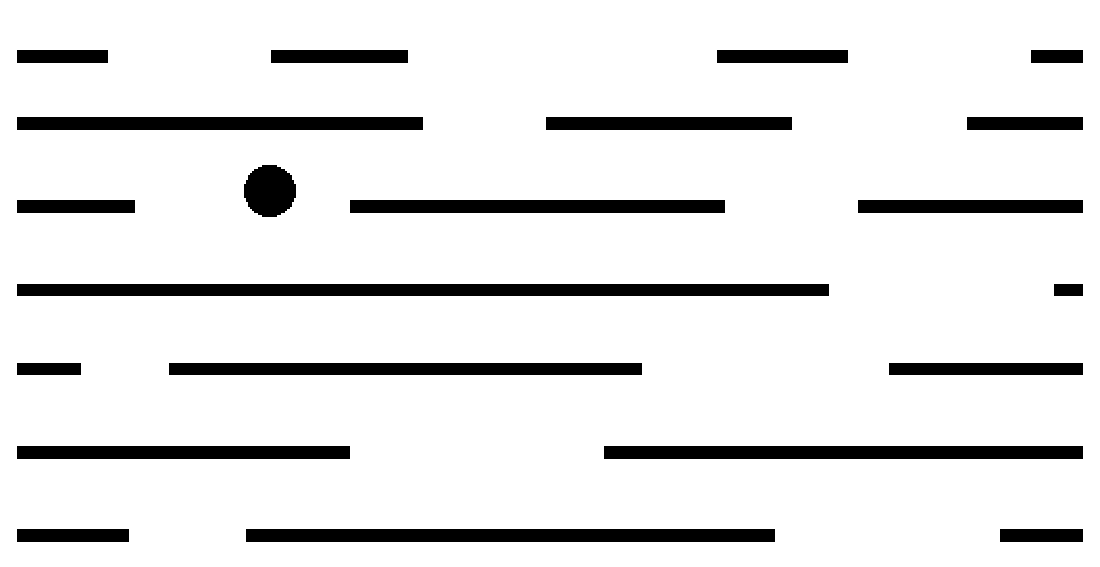
\includegraphics[width=4.5in]{example_screen.eps}
      \caption{An example game screen.}
   \end{center}
\end{figure}

\subsection{Loser Screen}

This screen appears after the player loses. It displays a message notifying
the user that they have died. Any keypress allows the user to proceed back to
the title screen to begin a new game. There is no cake at the end of the game.

\end{document}
